\section{Réseau Neuronal Convolutif}
Les réseaux neronaux convolutifs (ou Convolutional Neural Network)\cite{cnn} sont des réseaux de neurones qui utilisent des opérations de réduction de dimension et de convolution afin d'extraire des caractéristiques sur les données.\\

\subsection{Pré-traitement des Données}
Ces réseaux de neurones sont généralement associés à un réseau dense pour efféctuer la prédiction après avoir extrait les informations des données. Dans le cadre du projet, la prédiction correspond à une classe (genre du film) parmi neuf à l'aide du titre et du synopsis du film. La dernière couche du réseau comport donc neuf cellules qui donneront chacune la probabilité que le film appartienne à chaque classe. Pour l'apprentissage et la prédiction, il faut lister tous les genres, leur associer un indice et remplacer les valeurs dans les données (voir dictionnaires \textsf{genre2id} et \textsf{id2genre}).\\
Dans le dataframe, les colonnes \textit{titre} et \textit{synopsis} doivent être fusionnées afin de pouvoir les vectoriser dans la suite.

\subsection{Indexation du Vocabulaire}
Les réseaux neronaux convolutifs effectuent des opérations sur des données numériques. Pour une application en TAL, il faut transformer le contenu sous forme de texte en données numériques, par exemple représenter chaque mot comme un vecteur de nombres réels dans un espace de grande dimension.\\
Dans le programme, l'objet de type \textsf{TextVectorization} de la bibliothèque Tensorflow \cite{tensorflow} permet d'effectuer la vectorisation, chaque mot correpond alors à son indice dans le vecteur. Par exemple: si \textsf{TextVectorization} place le mot \textit{bonjour} à la troisième position du vecteur alors le mot \textit{bonjour} sera traité par le CNN comme la donnée 2.

\subsection{Chargement de Plongements de Mots Pré-entraînés}
La vectorisation des mots du vocabulaire est une opération complexe mais il est possible d'utiliser des plongements pré-entraînés.\\
Dans ce projet, le plongement \textit{frWiki\_no\_phrase\_no\_postag\_700\_cbow\_cut100.bin} \cite{fauconnier} de dimension 700 a été utilisé pour vectoriser les données.

\subsection{Construction et Entraînement du Réseau Neuronal Convolutif}
Un CNN est composé de plusieurs couches effectuant différentes opérations (réduction de dimension, convolution, couches denses). Le réseau utilisé dans ce projet contient seulement deux couches de réduction de dimension et deux couches de convolution (Figure \ref{architecture_cnn}).

\begin{figure}
    \center
    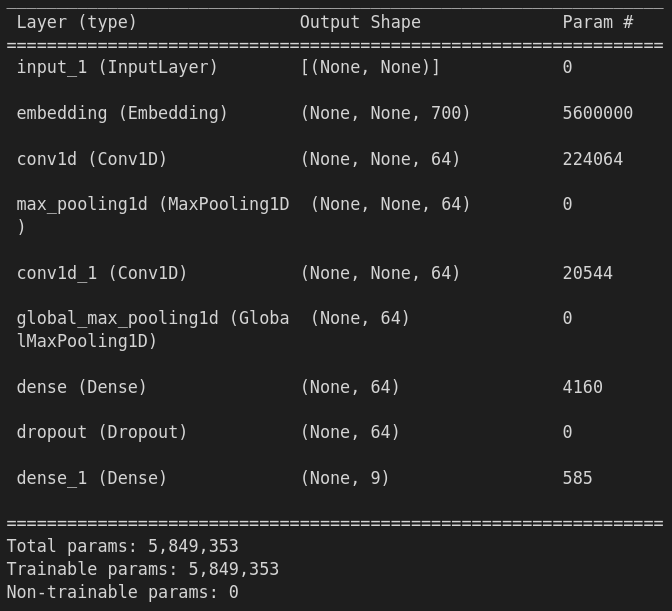
\includegraphics[scale=.3]{img/architecture_cnn.png}
    \caption{Architecture du réseau neuronal convolutif}
    \label{architecture_cnn}
\end{figure}

\noindent
\begin{minipage}[!hc]{0.12\textwidth}
   \textbf{Remarque}
\end{minipage}
\vrule\enskip\vrule\quad\begin{minipage}{\dimexpr 0.87\textwidth-0.8pt-1.5em}
Après plusieurs expériences avec différentes architectures, il semblerait qu'ajouter des couches de réduction de dimension et de convolution n'améliorent pas la qualité des résultats dans le cadre de cette étude.
\end{minipage}

Les opérations de convolution du CNN sont des opérations qui doivent être apprises au cours de l'entraînement. \cite{convolution} La taille des batchs est de 64 et le nombre d'epochs choisi est 25, permettant un apprentissage plus précis mais aussi plus long. Pour contrer cela, un callback de type \textsf{EarlyStopping} a été ajouté (arrêt de l'apprentissage lorsque la précision du modèle diminue).\\
Le réseau neuronal convolutif obtenu a une précision de 72.91\%.

\begin{figure}
    \center
    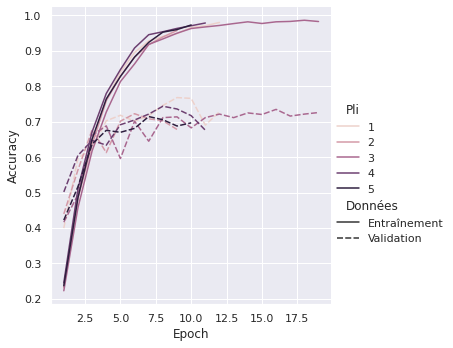
\includegraphics[scale=.3]{img/accuracy_cnn.png}
    \caption{Précision du réseau neuronal convolutif au cours de l'entraînement}
    \label{accuracy_cnn}
\end{figure}